\documentclass[a4paper]{article}
\usepackage[14pt]{extsizes}
\usepackage[utf8]{inputenc}
\usepackage[russian]{babel}
\usepackage{setspace,amsmath}
\usepackage[left=20mm, top=15mm, right=15mm, bottom=15mm, nohead, footskip=10mm]{geometry}
\usepackage{hyperref}
\hypersetup{
    colorlinks,
    citecolor=black,
    filecolor=black,
    linkcolor=black,
    urlcolor=black
}
\usepackage{graphicx}
\graphicspath{{./}}
\graphicspath{{./pictures/}}
\DeclareGraphicsExtensions{.pdf,.png,.jpg}
\usepackage[tableposition=top,singlelinecheck=false]{caption}
\usepackage{subcaption}
\DeclareCaptionLabelFormat{gostfigure}{Рисунок #2}
\captionsetup*[figure]{labelformat=gostfigure, justification=centering}
\usepackage{amsfonts}

\begin{document}
 
\begin{center}

\includegraphics{MSU}

\hfill \break
\normalsize{Московский государственный университет имени М.В. Ломоносова}\\
\normalsize{Факультет вычислительной математики и кибернетики}\\
\normalsize{Кафедра информационной безопаснсти}\\
\normalsize{Лаборатория безопасности информационных систем}\\
 \hfill \break
\normalsize{Николайчук Артём Константинович}\\
\hfill\break
\hfill \break
\hfill \break
\hfill \break
\large{Обзор методов fuzz-тестирования программ, принимающих на вход
данные, порождаемые КС-грамматикой}\\
\hfill \break
\hfill \break
\hfill \break
\normalsize{Курсовая работа}\\
\hfill \break
\hfill \break
\hfill \break
\hfill \break
\hfill \break
\hfill \break
\hfill \break
\hfill \break
\begin{flushright}
    \normalsize{Научный руководитель:}\\
    \normalsize{м.н.с}\\
    \normalsize{А.А.Петухов}\\
\end{flushright}
\end{center}
\vspace*{\fill}
\begin{center} Москва, 2022 \end{center}
\thispagestyle{empty}
 
\newpage
\section*{Аннотация}
\indent

В настоящее время разработчики всё больше беспокоятся о безопасности создаваемых приложений. Цена ошибки или бага может очень высокой. Тестирование стало неотъемлемой частью жизненного цикла разработки программного обеспечения. Некоторые програмы, такие как парсеры, интерпретаторы, компиляторы, обрабатывают данные, которые имеют сложную структуру. Вручную написать тесты с приемлемым покрытием для этих программ не представляется возможным. Для них разумно применять методы
генерации тестов, а также fuzz-тестирования поверх этих методов для
поиска ошибок. Эти методы подлежат обзору для того, чтобы оценить их
применимость для поиска недостатков безопасности шаблонизаторов.
\newpage
    \tableofcontents
\newpage
 
\newpage
\section{Введение}

\subsection{Fuzz-тестирование}
\indent

Fuzz-тестирование - способ автоматического тестирования программного обеспечения. Фаззер генерирует случайные входные данные и улучшает, или изменяет их, затем анализирует работу программы на этих данных, и пытается обнаружить потенциальные дефекты или уязвимости программного обеспечения. Фаззеры принято классифицировать по принципу генерации данных:

\begin{itemize}
\item Мутационные фаззеры обрабатывают заранее подготовленное множество входных данных. Наиболее популярными изменениями являются заимствованные из биологии мутации и скрещивания. Мутации - это изменение какой-то части входных данных на случайную. При скрещивании выбираются два примера, которые обмениваются друг с другом частью данных.
\item Генерационные фаззеры создают новые примеры, основываясь на информации о требуемой структуре входных данных. 
\item Смешанные фаззеры объединяют в себе два предыдущих подхода. Например, при мутации данные могут меняться не на случайные, а на сгенерированные. Или фаззер может сначала создать пул тестовых данных и к нему применять мутационный метод. 
\end{itemize}

\subsection{Представление входных данных}
\indent

На практике оказалось очень удобно задавать структуру входных данных с помощью грамматик (Пример грамматики на рис. \ref{SimpleGrammar}). Если известна грамматика, то все возможные входные данные можно представить абстрактным синтаксическим деревом (далее АST - Abstract Syntax Tree). Пример AST представлен на рисунке \ref{SimpleAST}. Это позволяет избегать синтаксических ошибок на этапе запуска программы. В дальнейшем будет показано, что такое представление полезно при генерации и мутации данных.

\begin{figure}[ht!]
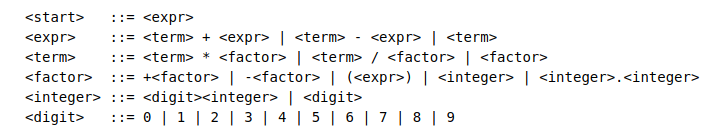
\includegraphics[width=180mm]{Expressions_Grammar.png}
\caption{Грамматика арифметических выражений}
\label{SimpleGrammar}
\end{figure}

\begin{figure}[ht!]
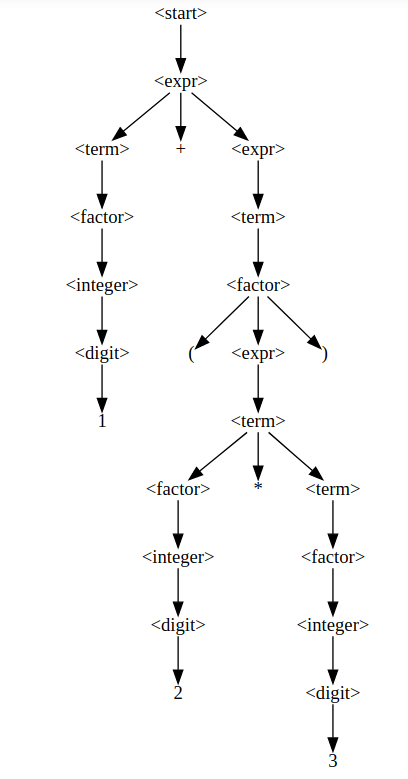
\includegraphics[width=100mm]{SimpleAST.png}
\caption{AST для выражения 1 + (2 * 3)}
\label{SimpleAST}
\end{figure}

\newpage
\section{Цель работы}
\indent

Цель данной работы - сделать обзор значимых методов и средств, используемых при fuzz-тестировании программ, обрабатывающих структурированные входные данные. Для достижения этой цели требуется:

\begin{itemize}
\item Сформировать критерии для сравнения методов.
\item Проанализировать существующие решения по выделенным критериям.
\item Дать оценку каждому критерию.
\end{itemize}

\newpage
\section{Анализ предметной области}
\indent
 
Базовый алогоритм работы любого фаззера состоит из шагов:

\begin{enumerate}
    \item Предобработка тестируемого программного обеспечения(далле SUT - Soft Under Test). Например, она может заключаться в компиляции со специальными флагами или подготовке окружения для тестирования. 
    \item Получить начальное множество входных данных и создать из него пул тестов.
    \item Выбрать из пула один или несколько примеров и получить результат их тестирования в SUT.
    \item Решить будет ли полезен этот тест в будущем.
    \item Мутировать тест и добавить его в пул.
    \item Перейти к шагу 3.
\end{enumerate}

\subsection{Получение начального множества тестов}
\indent

Первый способ получения входных данных - использовать тесты, которые написали разработчики для SUT. Этот способ позволяет сразу получить хорошее покрытие кода. При обнаружении бага разработчики исправляют его и часто добавляют тест, который проверяет работоспособность программы в этом месте. В этом смысле тесты, как начальное множество, позволяют сразу добираться до "слабых" мест в SUT. Минус этого способа - тесты разработчиков не всегда доступны.
\indent

Второй вариант - собрать пул тестов из примеров в интернете. Например, в случае fuzz-тестировании интерпретатора javascript можно в начальное множество добавлять примеры javasrcipt кода с гитхаба. Таким способом можно получить широкий пул тестов.
\indent

Третий - можно сгенерировать множество самостоятельно. В этом случае появляется возможность подтолкнуть фаззер в определённом направлении. Детали процесса генерации описаны ниже.

\subsection{Генерация тестов}
\indent

\subsubsection{Способы генерации}
\indent

Алгоритм создания тестовых данных опирается на знание их структуры. Как было отмечено ранее, эту структуру удобно задавать контекстно-свободной грамматикой. В этом случае процесс генерации нового теста заключается в построении его AST. Шаги алгоритма:

\begin{enumerate}
    \item Положить в корень дерева стартовую вершину и добавить её в очередь вершин.
    \item Взять текущую вершину из очереди.
    \item Если текущая вершина - терминальная, то перейти к следующей вершине.
    \item Каким-то способом выбрать продукцию из правила вывода для текущего нетерминала и добавить все символы из неё в очередь.
    \item Перейти к шагу два.
\end{enumerate}

Все известные методы опираются при выборе продукции нетерминала в пункте 4 на вероятности, то есть каждой продукции каждого нетерминала задаётся вероятность её выбора. Разные алгоритмы отличаются друг от друга способом задания этой вероятности. 

\begin{itemize}
\item Выбирать продукцию равновероятно для каждого нетерминала. Плюсы - простая реализация. Минусы - часто будут генерироваться похожие тесты, медленно покрываюся всевозможные ветки деревьев. Например: если у стартового символа одна из продукций - один терминальный символ, то большая часть сгенерированных тестов будет состоять из этого символа.
\item Алгоритм построения похожих\cite{litlink1}. Если имеется какое-то множество примеров, то каждый из них представляется в виде AST и для каждого нетерминала для каждой продукции подсчитывется частота её встречаемости. По этим частотам можно вычисляется вероятность выбора каждой продукции. Чем чаще встречается переход в тестах, тем чаще он будет использоваться. Плюсы - этот метод позволяет направлять фаззер, путём изменения множества. Выбор символа становится более осмысленным с точки зрения программирования. Минусы - требуется начальное множество тестов.
\item Алгоритм построения отличных. Отличие этого способа от предыдущего - вероятность выбора становится обратно пропорциональна частоте встречаемости, то есть чем чаще встречается переход в тестах, тем реже он будет генерироваться. Это позволяет двигаться фаззеру в противоположном направлении. Плюсы - чаще будут встречаться неожиданные пути в грамматике. Минусы - чаще будут попадаться неинтересные символы. Например, в javascript часто будет вызываться return. 
\item Ещё один способ - задать вероятности пропорционально количеству возможных поддеревьев в продукции. Если в вершине потенциально много поддеревьев, она будет чаще выбираться.
Плюсы - позволяет наиболее полно покрыть грамматику. 
Минусы - требуется предпосчёт количества деревьев для каждого нетерминала.
\end{itemize}

\subsubsection{Свойства сгенерированных тестов}
\indent

Сгенерированные тесты должны не только быть синтаксически корректными, но и обладать полезными для fuzz-тестирования свойствами.

\begin{itemize}
\item Нужно стремиться создавать короткие тесты. Чем тест длиннее - тем дольше он будет выполняться в SUT, тем сложнее его анализировать, тем дольше будет его обработка. 
\item Чем тест сложнее и рекурсивнее, тем вероятнее найти на нём ошибку SUT. 
\end{itemize}

Эти свойства не противоречат друг другу. Рассмотрим примеры для грамматики с рисунка \ref{SimpleGrammar}. Выражение "5+5+5+5+5+5+5+5+5+5+5+5" является длинным, но не сложным. Скорее всего при парсинге будет вызвана функция обработки знака "+" несколько раз последовательно, что лишь увеличит время работы программы. Другой пример - выражение "(5 + (5) + ((5 + 5) + 5))". Оно короче предыдущего, но при обработке скобок некоторые функции будут вызваны рекурсивно, что увеличивает вероятность найти ошибку.

\subsection{Получение обратной связи от запуска теста на SUT}
\indent

Получение обратной связи от запуска теста - важная часть фаззера. Именно она часто позволяет определять значимость входного набора данных. Метрики, которые полезно оценивать:

\begin{itemize}
\item Самая весомая метрика - возникновение в SOT искомых исключений,
например double free в языке программирования c++. Зачастую такие ошибки означают, что найден баг и этот тест нужно дополнительно исследовать вручную.
\item Покрытие кода(line coverage) и покрытие функций(function coverage) - подсчёт количества строк/функций, которые покрыл тест. В контесте множества тестов можно выявлять те, которые попадают в новые строки/функции. Разным строкам и функциям можно давать разный вес при подсчёте метрики. Это позволяет направлять фаззер в сторону исследования этих функций.
\item Покрытие веток(путей) - более сложный вариант предыдущей метрики. При подсчёте учитывается последовательность выполнения строк кода или вызывов функций. Плюсы - покрытие веток гораздо более информативная метрика, чем предыдущая. Минусы - число веток растёт очень быстро с увеличением количества кода в SUT.
\end{itemize}

\subsection{Оценка полезности теста}
\indent

После запуска теста требуется узнать полезен ли этот тест или от него можно отказаться. Для этого нужно научиться сравнивать различные входные данные друг с другом.
Для этого введём функцию $value : \mathbb {X} \rightarrow \mathbb {R}$, которая каждому тесту ставит в соответствие его численную оценку. Конкретных реализаций этой функции может быть много. Приведём основные параметры, от которых она может зависеть:
\begin{itemize}
    \item При наличии исключения при запуске, значение функции становится бесконечным.
    \item Чем больше покрытие кода, тем больше значение функции. Если тест покрывает новый участок кода, то функцию можно сделать равной бесконечности.
    \item Чем короче тест, тем больше значение функции.
    \item Чем тест разнообразнее, то есть чем больше символов грамматики он покрывает, тем лучше.
\end{itemize}

\subsection{Способы обработки тестового множества}
\indent

Существует две стратегии обработки тестового множества:

\begin{enumerate}
\item Первая - наиболее часто встречающаяся - обрабатывать каждый тест по отдельности. Это позволяет распараллелить процесс fuzz-тестирования, что серьёзно его ускоряет. 
\item Вторая стратегия основана на теории эволюции Дарвина. Выбирается множество тестов. Для них всех рассчитывается функция полезности. Затем начинается процесс "выживания". Какой-то процент (например 10) тестов с наибольшей функцией полезности объявляется выжившими. Остальные случайным образом делятся на группы, в которых выживает несколько сильнейших. Потом среди оставшихся несколько случайных тестов объявляются выжившими. Тесты, которые не выжили отбрасываются.
\end{enumerate}

\subsection{Методы улучшения тестов}
\indent

Все успешные тесты необходимо преобразовывать для продолжения процесса fuzz-тестирования. Целями улучшения могут быть: 
\begin{itemize}
\item Поиск наиболее оптимального теста с точки зрения фаззера, обладающего теми же свойствами, что и улучшаемый. Другими словами - оптимизация процесса fuzz-тестирования.
\item Дальнейшее продвижение фаззера, в том числе выход из локальных экстремумов.
\end{itemize}

\subsubsection{Уменьшение размера теста}
\indent

Как было отмечено ранее, у коротких тестов есть ряд преимуществ по сравнению с длинными. Уменьшенный тест должен сохранить все полезные свойства длинного. Например, если старый тест покрывает какую-то новую функцию, то и новый должен покрывать эту функцию. Стандартные методы минмизации:

\begin{itemize}
\item Самый простой способ заключается в построении AST теста и поочерёдном удалении поддеревьев. Если после удаления поддерева, полезность теста не уменьшилась, то старый тест заменяется на новый, и продолжается процесс минимизации. Плюсы - неплохая скокорость работы. С небольшой вероятностью тест  существенно укоротится. Минусы - удаление поддерева может сделать тест синтаксически некорректным. Этот способ охватывает только очень локальные изменения теста.
\item Уменьшение поддерева. Способ похож на предыдущий, только вместо отбрасывания поддерева, оно заменяется на более короткое. Новый тест всегда будет синтаксически корректным, но перебор всех поддеревьев может занять длительное время.
\item Рекурсивное замещение поддерева. По сути этот способ является эвристикой предыдущего. Если в вершине у нетерминала F есть сын F, то производится замена поддерева текущей вершины на поддерево сына. Такое изменение оставит тест синтаксически корректным и приведёт к его упрощению для фаззера. Минус - этот способ может быть редко применим.
\item Контролировать размер во время построение теста. Этот способ применим, если используется генерация тестов. Тогда этап уменьшения можно опустить.
\end{itemize}

\subsubsection{Мутации}
\indent

Мутации являются двигателем фаззера, позволяют ему эволюционировать. Если фаззер "застрял" на каком-то этапе, то мутации могут сделать шаг в сторону и процесс fuzz-тестирования продолжится. Если тесты представимы в виде AST, то удобно описывать мутации изменениями над AST. 

\begin{itemize}
\item Скрещивание тестов друг с другом. Берустя два успешных теста, представляются в виде AST, и поддерево одного теста заменяется на поддерево другого согласно правилам грамматики. Такое изменение, например, позволяет быстро увеличивать покрытие веток SUT.   
\item Создаётся пул поддеревьев. Для каждой вершинки в AST теста считается  какая-то дополнительная информация. Поддерево этой вершинки может быть заменено только на поддерево из пула с такой же информацией. Например, информацией может быть тип нетерминала, количество идентификаторов. В пул тестов добавляются поддеревья из тестов, которые дают существенное улучшение полезности. Эта мутация позволяет обращать больше внимания на прогресс в фаззере. Например, если тестом покрыта какая-то новая функция, то среди новых тестов будет много тех, которые эту функцию исследуют. Сохранение дополнительной информации позволяет увеличить вероятность попадания в новую функцию.
\item Рекурсивное дублирование поддерева. Это обратное действие одному из способов уменьшения. Эта мутация направлена на усложнение структуры выполняемого кода в SUT, например, на создание вложенных циклов или рекурсии. 
\item Применимы стандартные AFL мутации - бит флип, замена "интересных значений". Они более случайны, их имеет смысл применять, когда остальные не работают. После применения этой мутации тест может стать синтаксически некорректным.
\item Замена поддерева на случайно сгенерированное. Эта мутация - адаптированная для fuzz-тестирования с грамматикой версия предыдущего пункта. Основное отличие - тест останется корректным.
\item При использовании метода генерации тестов по вероятностной грамматике можно изменять вероятности генерации продукции для конкретного нетерминала. Можно изменять на случайные, можно просто немного прибавить или отнять вероятности у нескольких символов. Новые тесты могут сильно отличаться от предыдущих. Плюс такой мутации - не нужно работать с самими тестами, достаточно просто изменить вероятность при генерации.  
\end{itemize}


\newpage
\section{Анализ инструментов предметной области}
\indent

Цель анализа - рассмотреть работу инструментов, которые применяются при fuzz-тестировании программ или решают задачу генерации входных данных. В обзоре рассмотрены самые цитируемые актуальные статьи с google scholar.

\subsection{Superion}
\indent

Superion\cite{litlink3} - grey-box fuzzer, созданный на основе AFL. Является линией отсчёта для остальных рассматриваемых фаззеров. Разбор Superion по критериям: 
\begin{enumerate}
    \item Подразумевается, что начальный пул тестов уже имеется.
    \item Генерация тестов не используется.
    \item В Superion используется стандартное покрытие AFL - покрытие веток. В реализации происходит подсчёт всех веток, которые покрыл тест, и количество проходов по ним.
    \item Функция полезности - при увеличении покрытия, тест обозначается успешным.
    \item Каждый тест обрабатывается по отдельности.
    \item Улучшение тестов:
    \begin{itemize}
        \item Для уменьшения размера тестовых данных используется самая простая стратегия - удаление поддеревьев. В статье делается следующий вывод: "Таким образом, несмотря на относительно низкий коэффициент обрезки, эта стратегия обрезки с учетом грамматики может значительно улучшить коэффициент валидности для тестовых входных данных после обрезки, что облегчает и ускоряет дальнейшую работу с ними."
        \item Используется мутация скрещивания тестов. Реализация: берётся текущий тест и случайный из очереди длины не более 10000 байт. Они парсятся и из их поддеревеьев формируется множество для мутаций. Берётся не больше 10000 поддеревеьев и длина не более 200 байт.
        Затем каждое поддерево текущего теста заменяется на каждое поддерево из множества, формируя новый тест.\\
        Плюсы: очень подробный перебор возможных тестов.\\
        Минусы: несмотря на ограничения тестов получается очень много. Довольно большая проблема фаззера - время подготовки данных. Если программа выполняется t секунд, то время на мутации примерно t/3.
        \item Применяется мутация замены по словарю. В каждое корректное, согласно грамматике, место вставляется значение из множества стандартных для грамматики конструкций. Делается предположение, что все токены должны состоять из цифр и букв. Словарь токенов можно либо составить вручную, либо взять самые популярные токены из множества тестов. При мутации новый токен либо вставляется между двумя старыми, либо заменяет один из них.
    \end{itemize}
    В статье сравнивали различные мутации. Самыми удачными оказались мутация замены поддеревьев и перезапись токенов при помощи словаря, определённого человеком.
\end{enumerate}
Superion хорошо себя показал при сравнении с обычным AFL и jsfunfuzz - специальным фаззером для js. Тестирование проводилось на парсерах xml и интерпретаторах javascript.

\subsection{Grammarinator}
\indent

Grammarinator\cite{litlink5} - инструмент, позволяющий генерировать тестовые данные по имеющейся грамматике. Так как это неполноценный фаззер, имеет смысл описать только некоторые критерии.

\begin{enumerate}
\item При создании тестов используется равновероятная грамматика с небольшими улучшениями. После выбора какого-то правила вероятность его повторного выбора уменьшается. Такой подход помогает направлять
поколение к менее посещаемым частям грамматики. Во премя генерации контролируется размер тестов. Для каждого символа грамматики производится предподсчёт минимального размера поддерева и при генерации выбираются только те символы, поддеревья которых не превысят заданную длину теста. В Grammarinator используется алгоритм переиспользования токенов. Это позволяет уменьшить количество тестов с семантическими ошибками. Например, при fuzz-тестировании интерпертатора javascript будет сгенерировано меньше тестов с ошибкой "использование необъявленной переменной".
\item Создаётся пул тестов, которые используются для ускорения создания тестовых примеров с помощью эволюционных методов. Одна из возможностей заключается в выполнении случайной рекомбинации деревьев из пула для создания новых тестовых примеров. Другой вариант - деревья из пула используются, как поддеревья генерируемых тестов.
\end{enumerate}


\subsection{Nautilus}
\indent
Nautilus\cite{litlink6} - фаззер, сочетающий в себе способность генерировать входные данные по грамматике и ориентироваться на покрытие кода. Разбор Nautilus по критериям:

\begin{enumerate}
\item Начальный пул тестов не нужен.
\item Тестировались два варианта генерации: равновероятный по грамматике и равномерный по количеству возможных поддеревьев. В статье методы тестировали на разных интерпретаторах: для некоторых лучше работал второй метод, для некоторых одинаково.
\item Используемая метрика - покрытие строк кода.
\item Функция полезности - при увеличении покрытия, тест обозначается успешным.
\item Тесты обрабатываются по отдельности.
\item Улучшение тестов:
    \begin{itemize}
        \item Используется две стратегии уменьшения тестов. Минимизация поддерева - для каждого нетерминала изменяется поддерево на минимально возможное поддерево в этом нетерминале и проверяется покрытие. Далее применяется рекурсивная минимизация. Её цель состоит в том, чтобы уменьшить количество рекурсий, заменяя их по одной за раз. Из этих стратегий лучше работает первая.
        \item К каждому тесту применяется одна из следующих мутаций. 
        \begin{enumerate}    
        \item Случайное поддерево изменяется на случайно сгенерированное поддерево.
        \item Каждая вершина меняется на дерево, сгенерированное по смежным правилам.
        \item Рекурсивная мутация - если у нетерминала, есть сын, совпадающий с нетерминалом, повторяем его $ 2^n $ раз, $ n $ - небольшое.
        \item Скрещивание деревьев. Скрещивание происходит только между тестами, покрывающими новые участки кода.
        \item Мутации АФЛ.
        \end{enumerate}
        В начале процесса fuzz-тестирования лучше всего себя показывает первый тип мутаций. Через некоторое время скрещивание обгоняет его.
    \end{itemize}
\end{enumerate}

\subsection{EvoGFuzz}
\indent

В EvoGFuzz\cite{litlink2} идея строить тесты по грамматике с вероятностями является ключевой. Удалось спроектировать фаззер так, что почти весь код является реализацией генерации теста. Мутации опираются на вероятности в грамматике. 
\begin{enumerate}
    \item Требуется множество тестов для создания грамматики с вероятностями.
    \item Для генерации входных данных используется грамматика с вероятностями. При создании контролируется размер входных данных. 
    \item При запуске теста требуется получать только информацию об исключениях.
    \item Функция полезности выглядит следующим образом:\\
    $f(x) = \infty$ , если тест упал с ошибкой\\
    $f(x) = expansions(x) ^ 2 / length(x) $,\\
    $expansions(x)$ - количество расширений(нетерминальных символов) \\
    $length(x)$ - длина теста в символах.\\
    Использование такой функции позволяет более сложным тестам получать большую полезность, а длинные тесты штрафуются. 
    Плюсы: функция просто вычисляется, учитывает свойства, которые требуется получить от теста.
    Минусы: Тесты могут получаться длинными в терминах грамматики.
    \item Используется стратегия эволюции тестов. Запускается всё множество тестов и для каждого вычисляется функция полезности. Остаётся примерно 5\% тестов, с максимальной функцией качества. Среди не вошедших в топ 5\% случайным образом формируется 10 групп по 10 тестов, и победители остаются для дальнейшей работы.
    \item Единственная мутация - для каждого нового поколения выбирается случайный нетерминал в грамматике, и вероятности перехода из него меняются на случайные.
\end{enumerate}

\subsection{Выводы}
\indent

Для fuzz-тестирования шаблонизаторов предлагается использовать наиболее отличившиеся идеи. Среди будущих мутаций обязательно должны присутствовать скрещивание и замена поддерева на случайное, потому что они выделяются среди остальных. Для генерации тестов можно использовать алгоритм построения похожих, вероятности вычислить по реальным программам. Для борьбы с семантическими ошибками можно использовать идеи из Grammarinator. Среди стратегий обработки тестов нет явно выделяющейся, но идеи, описанные в EvoGFuzz, мало изучены, предлагается исследовать именно их.

\newpage
\section{Результаты}
\indent

В рамках данной работы были получены следующие результаты:
\begin{itemize}
    \item Сделан обзор методов fuzz-тестирования программ, принимающих на вход данные, порождаемые КС-грамматикой. Выделены критерии для сравнения таких фаззеров.
    \item Произведён анализ существующих инструментов. На его основе предложен алгоритм для fuzz-тестирования шаблонизаторов.
\end{itemize}

\newpage

\begin{thebibliography}{}
    \addcontentsline{toc}{section}{Список литературы}
    \bibitem{litlink1}  Inputs from Hell Generating Uncommon Inputs from Common Samples [Электронный ресурс]. URL: \href{https://arxiv.org/pdf/1812.07525.pdf}{https://arxiv.org/pdf/1812.07525.pdf} (дата обращения: 18.05.2021)
    \bibitem{litlink2}  Evolutionary Grammar-Based Fuzzing [Электронный ресурс]. URL: \href{https://arxiv.org/pdf/2008.01150.pdf}{https://arxiv.org/pdf/2008.01150.pdf} (дата обращения: 18.05.2021)
    \bibitem{litlink3}  Superion: Grammar-Aware Greybox Fuzzing [Электронный ресурс]. URL: \href{https://arxiv.org/pdf/1812.01197.pdf}{https://arxiv.org/pdf/1812.01197.pdf} (дата обращения: 18.05.2021)
    \bibitem{litlink4}  Fuzzing With Optimized Grammar-Aware
    Mutation Strategies [Электронный ресурс]. URL: \href{https://ieeexplore.ieee.org/stamp/stamp.jsp?arnumber=9469897}{https://ieeexplore.ieee.org/stamp/stamp.jsp?arnumber=9469897} (дата обращения: 18.05.2021)
    \bibitem{litlink5}  Grammarinator:
    A Grammar-Based Open Source Fuzzer [Электронный ресурс]. 
    URL: \href{https://www.researchgate.net/publication/328510752\_Grammarinator\_a\_grammar-based\_open\_source\_fuzzer}{Grammarinator}
    (дата обращения: 18.05.2021)
    \bibitem{litlink6}  NAUTILUS:
    Fishing for Deep Bugs with Grammars [Электронный ресурс]. URL: \href{https://www.ndss-symposium.org/wp-content/uploads/2019/02/ndss2019\_04A-3\_Aschermann\_paper.pdf}{Nautilus} (дата обращения: 18.05.2021)
    \bibitem{litlink7}  The Fuzzing Book [Электронный ресурс]. URL: \href{https://www.fuzzingbook.org/}{https://www.fuzzingbook.org/} (дата обращения: 18.05.2021)
    \bibitem{litlink8}  Systematically Covering Input Structure [Электронный ресурс]. URL: \href{https://publications.cispa.saarland/2971/1/ase19-paper381-published.pdf}{https://publications.cispa.saarland/2971/1/ase19-paper381-published.pdf} (дата обращения: 18.05.2021)
\end{thebibliography}

\end{document}